\documentclass[a4paper, 12pt, -shell-escape]{article}  % тип документа
% русский язык

\usepackage[T1,T2A]{fontenc}  % кодировка
\usepackage[utf8]{inputenc}   % кодировка исходного текста
\usepackage[english,russian]{babel} % локализация и переносы
\usepackage{pdfpages}
\usepackage{minted}
\usepackage{geometry}

% геометрия
\geometry{pdftex, left = 2cm, right = 2cm, top = 2.5cm, bottom = 2.5cm}
\setcounter{tocdepth}{4} % фикс переноса 
\righthyphenmin = 2
\tolerance = 2048

% математика
\usepackage{amsmath, amsfonts, amssymb, amsthm, mathtools}

\begin{document}
	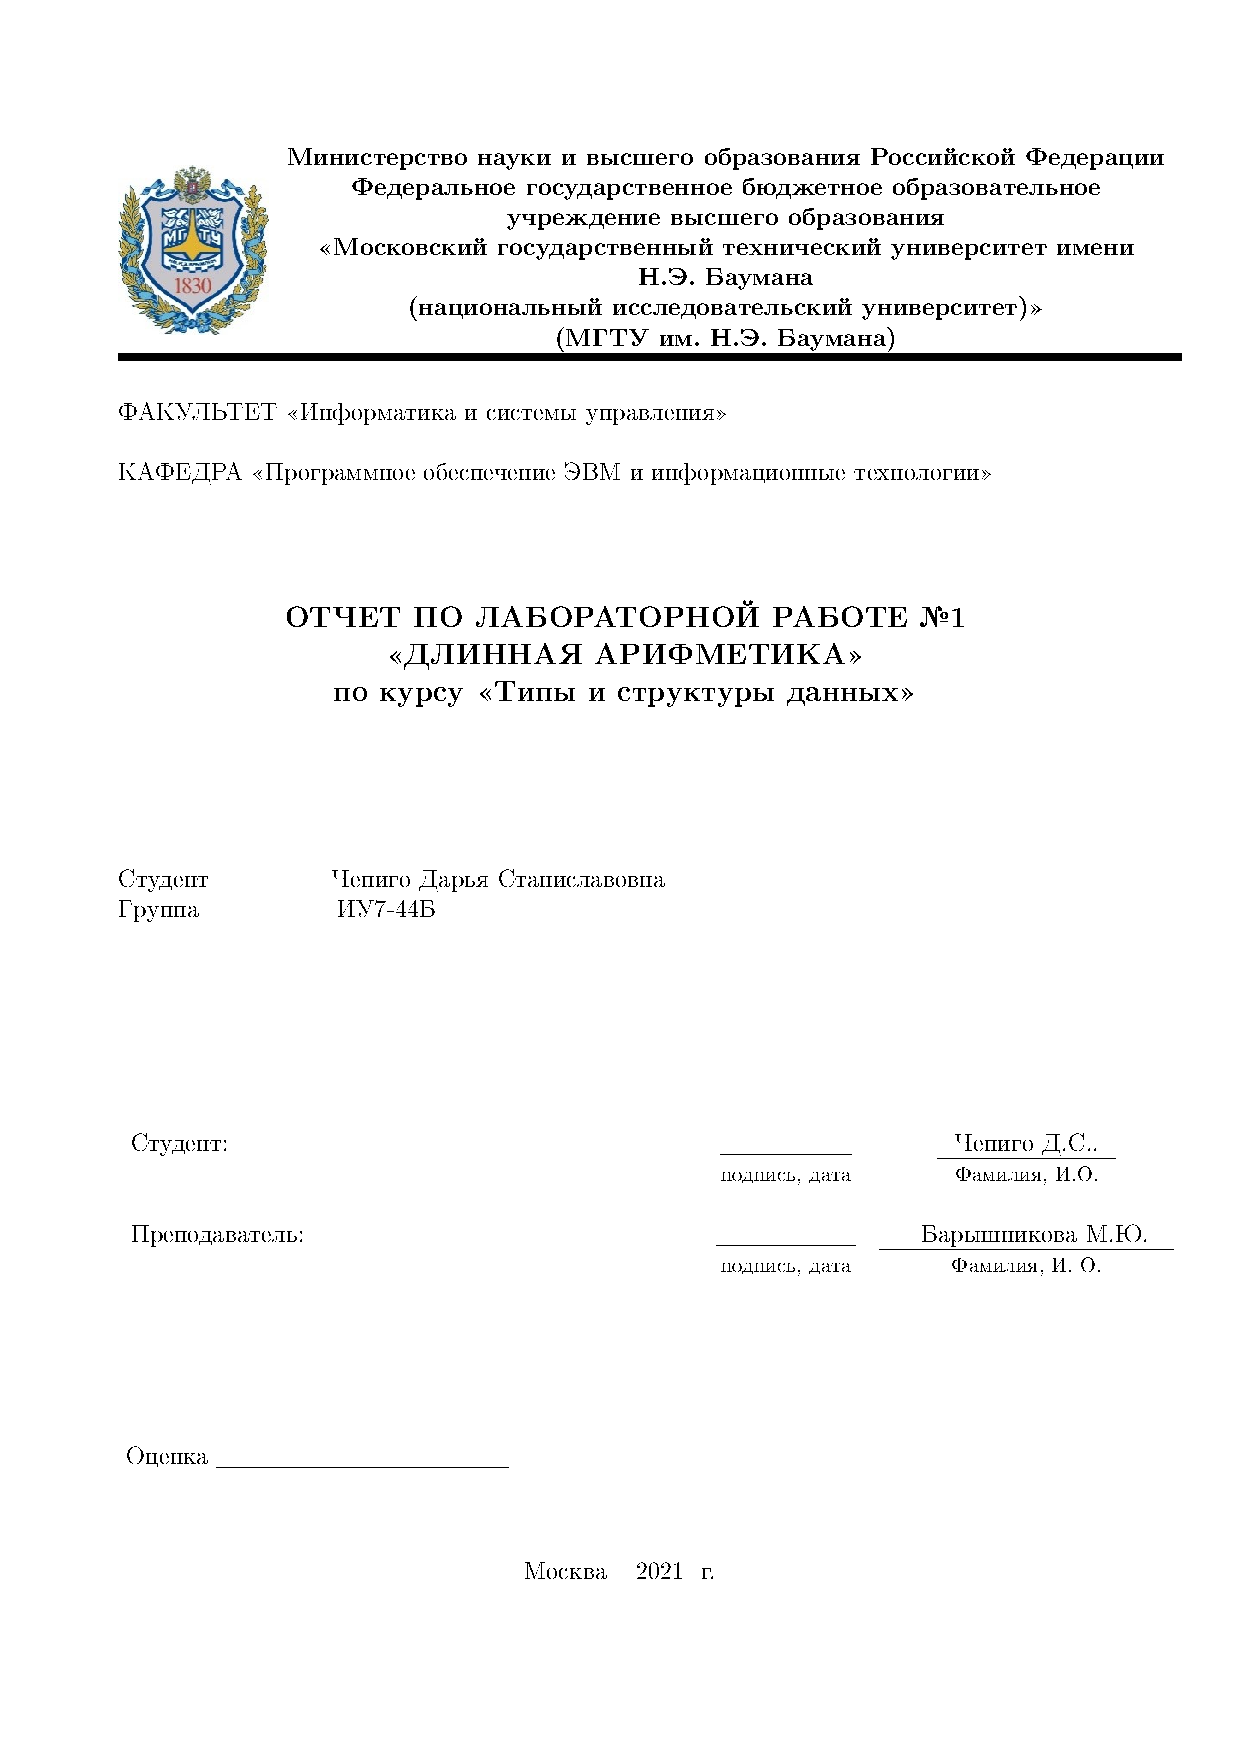
\includepdf{mrrvz.pdf}
	\newpage
	\begin{center}
	\begin{large}
		\textbf{Условие задачи}\\
	\end{large}
	\end{center}

	Смоделировать операцию умножения действительного числа в форме $\pm$ m.n Е $\pm$ K, где суммарная длина мантиссы (m+n) - до 30 значащих цифр, а величина порядка K - до 5 цифр, на целое число длиной до 30 десятичных цифр. Результат выдать в форме $\pm$ 0.m1 Е $\pm$ K1, где m1 - до 30 значащих цифр, а K1 - до 5 цифр.\\
	
	\begin{center}
		\begin{large}
			\textbf{Техническое задание}\\
		\end{large}
	\end{center}

	\textit{Входные данные}

	Одно действительное десятичное число, записанное в формате $[\pm]mmm.nnn[e][\pm]ppppp$
	(в квадратных скобках даны варианты символа на одной и той же позиции), где m, n, p – цифры, причем суммарное количество цифр до и после точки не превышает 30, число цифр после знака порядка не превышает 5 , а сам порядок по модулю меньше, чем 99999, буква «e» – латинские, знак <<+>> или <<->> у мантиссы и у порядка должен обязательно присутствовать. Ведущие нули в целом числе включаются в подсчет длины числа.
	Одно целое десятичное число, состоящее не более чем из 30 цифр, перед которыми обязательно должен быть знак <<+>> или <<->>.\\
	
	\textit{Выходные данные}
	
	Одно действительное число, записанное в формате $[\pm]0.mmmm[E/e][\pm]ppppp$
	(в квадратных скобках даны варианты символа на одной и той же позиции), где m, p – цифры, причем количество цифр в мантиссе не превышает 30, знак порядка может присутствовать, число цифр после знака порядка не превышает 5.\\
	
	\textit{Способ передачи входных данных}
	
	Входные данные передаются программе путем ввода в стандартный поток ввода на соответствующий запрос программы.\\
	
	\textit{Способ получения выходных данных }
	
	Выходные данные выводятся в стандартный поток вывода.\\
	
	\textit{Задача программы}
	
	Программа, получив на вход два числа, осуществляет их умножение и выводит результат в указанном формате. При невозможности получения результата программа выводит сообщение об ошибке.\\
	
	\textit{Способ обращения к программе }
	
	Обращение к программе осуществляется путем запуска исполняемого файла программы app.exe.\\
	
	\textit{Возможные ошибочные ситуации}
	\begin{enumerate} 
		\item Отсутствие одного или двух чисел в стандартном потоке ввода; 
		\item Некорректный ввод одного или двух чисел;
		\item Переполнение порядка результата.\\
	\end{enumerate}





	\newpage
	\begin{center}
	\begin{large}
		\textbf{Описание используемых структур данных}\\
	\end{large}	
	\end{center}
	
	\textit{Строка, содержащая число}
	
	Содержит символы, введенные пользователем. Для целого числа длина такой строки равна 32 (знак числа, 30 цифр, символ перехода на новую строку <<$\backslash$n>> и символ конца строки <<$\backslash$0>>), для вещественного – 41 (знак мантиссы, 30 цифр в мантиссе, точка в мантиссе, знак порядка, 5 цифр в порядке, символ перехода на новую строку <<$\backslash$n>> и символ конца строки <<$\backslash$0>>).
	
	\begin{minted}[fontsize=\footnotesize]{c}
	    char real_num[MAX_STR]; - строка для действительного числа(MAX_STR = 41)
	    char int_num[MAX_INT]; - строка для целого числа(MAX_INT = 33)
	\end{minted}

	\textit{Массив цифр}
	
	Для хранения результата произведения целого числа и мантиссы действительного числа используется массив цифр. Массив имеет длину 60. Это сделано для того, чтобы обеспечить корректность вычислений при переходе через десяток, когда длина мантиссы максимально допустимая. Каждая цифра имеет тип int, в связи с используемым алгоритмом. Цифры записываются в массив справа налево, то есть последняя цифра числа имеет индекс 0, предпоследняя 1 и т. д. Это сделано для удобства вычислений.
	
	\begin{minted}[fontsize=\footnotesize]{c}
	    int result[MAX_MULTI] = {0}; - массив для произведения двух чисел
	    (MAX_MULTI = 60)
	\end{minted}

	\textit{Структура «длинное вещественное»}
	
	Содержит строку, содержащую все число (со знаками, точками и символом экспоненты), знак мантиссы типа char, массив цифр мантиссы типа char, знак порядка типа char, значение порядка типа int и положение точки типа size\_t. Данные хранятся в одной структуре для обеспечения удобной совместной обработки всех данных.
	\begin{minted}[fontsize=\footnotesize]{c}
	struct real_number
	{
	    char real_num[MAX_STR]; - строка для действительного числа (MAX_STR = 41)
	    char sign_mantissa; - символ знака мантиссы
	    char mantissa[MAX_MANTISSA]; - строка для цифр мантиссы (MAX_MANTISSA = 32)
	    char sign_order; - символ знака порядка
	    int order; - массив, содержащий порядок
	    size_t point_place; - позиция точки в мантиссе
	};
	\end{minted}

	\textit{Структура «длинное целое»}
	
	Данная структура содержит знак целого числа типа char, массив его цифр типа char. Данные хранятся в одной структуре для обеспечения целостной обработки данных.
	\begin{minted}[fontsize=\footnotesize]{c}
	struct int_number
	{
	    char sign_int; - символ знака числа
	    char int_num[MAX_INT]; - массив, содержащий целое число (MAX_INT = 33)
	};
		\end{minted}






	\newpage
	\begin{center}
		\begin{large}
			\textbf{Описание алгоритма}\\
		\end{large}	
	\end{center}

	\textit{1.Ввод данных}
	
	При запуске программы на экран выводятся правила, которые надо соблюдать при вводе чисел. Если хотя бы одно из них не выполнено – программа выдаст ошибку. Ниже – пример программы с правилами и удобным примером для ввода.\\
	
	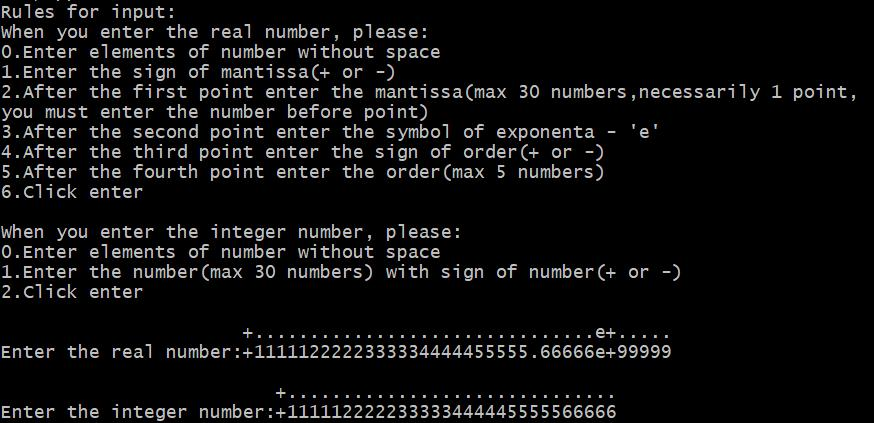
\includegraphics[width=\linewidth]{start}\\
	Считываем действительное и целое число в соответствующие строку из стандартного потока ввода. Если они считались успешно, то далее из строк записываем данные в соответствующие элементы структуры.\\
	
	\textit{2. Запись во внутренние структуры}
	
	Обрабатывая строку действительного числа по очереди проверяется все её содержимое, а именно наличие знаков, символа экспоненты, корректность мантиссы и порядка, находится позиция точки. После этого высчитывается порядок чисел и осуществляется нормализация. Далее удаляется точка в массиве чисел мантиссы для алгоритма умножения.
	
	Целое число аналогично проверяется на наличие знака и корректные цифры. Запоминается знак, цифры записываются в массив символов.
	Если в ходе обработки входных данных произошла ошибка, выводим сообщение и завершаем работу программы.\\
	
	\textit{3.Вычисления}\\
	
	\textit{Умножение двух чисел}

	Для алгоритма умножения двух чисел, размер которых максимум 30 цифр создаётся массив на 60 символов. Это реализуется с помощью двух циклов for с переменной i для первого числа и переменной j для второго числа соответственно. По очереди все цифры первого числа умножаются на все числа второго числа, их произведение записывается в ячейку массива под номером (60 – I - j). При этом после завершения этих циклов происходит проход по массиву с конца для переноса чисел, которые больше 10 в следующий разряд соответственно.\\
	
	\textit{Вычисление порядка}
	
	После того, как мы знаем количество значащих цифр в результате нашего умножения мы можем вычислить порядок по формуле =количество значащих цифр в результате – изначальный порядок действительного числа – количество цифр в действительном числе после точки. Если при округлении первой цифрой числа была “9” и это округлилось, то порядок меняется на 1.\\
	
	\textit{Корректировка мантиссы}
	
	Число знаков в мантиссе может превысить максимально допустимое. Найдем разницу между числом знаков результата и максимально допустимым. Если оно не положительно, корректировка не требуется. В противном случае сдвинем разряды результата так, что первая цифра займет 30-е справа место, предварительно запомнив цифру, идущую после первой справа сохраняемой цифры. Если запомненная цифра от 5 до 9, то прибавим 1 в последнем разряде мантиссы.\\
	
	\textit{Определение знака}
	
	Если два исходных числа имеют одинаковый знак, знак результата принимается равным «+», иначе – «-».\\
	
	\textit{4.Вывод результата или сообщения}
	
	Если в ходе обработки входных данных произошла ошибка, выводим сообщение и завершаем работу программы. Если ошибки нет, выводим результат в указанном выше формате.
	
	\newpage
	\begin{center}
		\begin{large}
			\noindent\textbf{Контрольные вопросы}\\
		\end{large}
	\end{center}
	\textit{1.Каков возможный диапазон чисел, представляемых в ПК?}
	
	Если под хранение целого положительного числа выделено 16 разрядов, то его максимальное значение не может превышать 216 – 1 = 65 535, если выделено 32 разряда, то максимальное значение составит 232 – 1 = 4 294 967 295. Для 64 разрядов максимально возможное значение числа равно 264 – 1 = 18 446 744 073 709 551 615.
	
	Вещественные числа представляются в виде мантиссы и порядка. Мантисса – правильная дробь, первая цифра которой отлична от нуля, т.е. находится в интервале [0.1, 1). Порядком – степень основания системы счисления, в которой сохранено число. 
	Длина мантиссы определяет точность представления числа, а длина порядка ограничивает диапазон допустимых значений. Максимально под представление мантиссы отводится 52 разряда в двоичной системе счисления, а под представление порядка – 11 разрядов. В этом случае возможные значения чисел находятся в диапазоне от 3.6 E –4951 до 1.1 E +4932.
	""\newline\newline
	\textit{2.Какова возможная точность представления чисел?}
	
	Целые числа хранятся в памяти ПК точно. Вещественные числа могут быть: одинарной точности, тогда точность составляет 7-8 значащих цифр после запятой; двойной точности с 15-16 значащими цифрами; четверной точности – около 34 значащих цифр.
	""\newline\newline
	\textit{3.Какие стандартные операции возможны над числами?}
	
	Набор операций над числом определяется его типом. Целые и вещественные числа поддерживают арифметические операции (сложение, вычитание, умножение, деление) и операции сравнения (кроме сравнения на равенство для вещественных чисел, их надо сравнивать, учитывая погрешность – некоторое маленькое число).
	
	Целые числа в языках подобных Си также поддерживают битовые операции (битовые И, ИЛИ, ИЛИ-НЕ, НЕ) и операцию взятия остатка от деления, отдельная операция для целочисленного деления. В некоторых языках программирования, реализована операция возведения в степень.
	""\newline\newline
	\textit{4.Какой тип данных может выбрать программист, если обрабатываемые числа превышают возможный диапазон представления чисел в ПК?}
	
	Программист может сохранить цифры числа в массиве или разбить число на части, каждую часть сохранить как отдельное число, обработать эти части и затем склеить их для выдачи результата пользователю.
	""\newline\newline
	\textit{5.Как можно осуществить операции над числами, выходящими за рамки машинного представления?}
	Можно сохранить числа в самостоятельно разработанном представлении, как в 4 вопросе, и обработать сохраненные таким образом числа с использованием операций над используемыми типами данных. Для четырех арифметических операций – сложения, вычитания, умножения, деления – существует алгоритм вычисления результата «столбиком», который несложно реализовать самим. Для операций сравнения можно использовать поразрядное сравнение.
	
	
	
	\newpage
	\begin{center}
		\begin{large}
			\noindent\textbf{Тестирование}\\
		\end{large}
	\end{center}
	
	Тут должно быть тестирование, но оно в 1 лабе было огромное, так как я скринила ВСЕ func тесты, которые выглядели как в си...
	
	Собственно так делать не надо и копировать сюда я это тоже не стала :з
	
	\newpage
	\begin{center}
		\begin{large}
			\noindent\textbf{Выводы}\\
		\end{large}
	\end{center}
	По итогам лабораторной работы заключаем следующее: 
	\begin{enumerate} 
		\item Целые и вещественные числа имеют различное хранение в памяти компьютера: целые – точно, а вещественные – приближенно (точность зависит от используемого типа данных).
		\item  Невозможно сохранить сколь угодно большое (маленькое) по модулю число со сколь угодно большой точностью. 
		\item В случае, если не удается использовать стандартные типы данных, то программист может самостоятельно решать этот вопрос разными способами.
		
	\end{enumerate}

	
\end{document}